\chapter{Klaidinantis SQLite klaidos pranešimas}

\section{Tikslas}

Iš taikomosios programos, naudojančios 
Django\footnote{Projekto svetainė: \url{https://www.djangoproject.com/}.} 
karkasą, įrašyti duomenis į
SQLite\footnote{Projekto svetainė: \url{http://sqlite.org/}.}
duomenų bazę.

\section{Priemonės}

Nustatymų faile buvo prašoma nurodyti failų sistemos kelią iki duombazės 
failo. Kadangi programa turėjo veikti GNU/Linux sistemoje, tai taip
pat buvo patikrinta, ar naudotojas, kuris paleidžia programą, turi
teisę skaityti ir rašyti nurodytą failą.

\section{Rezultatas}

Programa lūžo, su klaidos pranešimu nurodytu
\ref{fig:case_1_sqlite_error} paveiksle. Kadangi visi su duombaze susiję
nustatymai tėra tik kelias iki failo, tai reakcija buvo dar kartą
patikrinti ar programa pasiekia failą ir ar gali jį skaityti ir rašyti.
Kaip vėliau paaiškėjo, su pačiu duomenų bazės failu viskas yra gerai.
Duomenų bazė bando sukurti failą, informacijai apie tranzakcijas
saugoti, tame pačiame kataloge, kuriame yra ir pats duombazės failas,
bet to jai padaryti nepavyksta, nes naudotojas, paleidęs programą,
neturi tesės rašyti į tą katalogą.

\begin{figure}[H]
  \begin{center}
    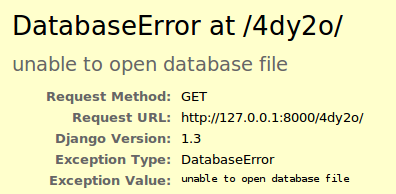
\includegraphics[width=0.4\textwidth]{images/case_1_sqlite_error.png}
  \end{center}
  \caption{Klaidinantis SQLite klaidos pranešimas}
  \label{fig:case_1_sqlite_error}
\end{figure}

\section{Panaudojamumo principas}

TODO

\section{Pamąstymai}

Galimas paaiškinimas, kodėl SQLite grąžina būtent tokį klaidos
pranešimą, būtų tai, kad tranzakcijų failas yra kuriamas bandant
atidaryti duomenų bazės failą ir įvykusios atidarymo metu klaidos
nėra diferencijuojamos. Vienas iš paprasčiausių sprendimų būtų
tiksliai nurodyti priežastį, kodėl būtent nepavyko atverti
duomenų bazės.
